\documentclass[a4paper, 14pt]{extarticle}
\usepackage[utf8]{inputenc}
\usepackage[paper=a4paper, top=1cm, right=1cm, bottom=1.5cm, left=2cm]{geometry}
\usepackage{setspace}
\onehalfspacing

\usepackage{graphicx}
\graphicspath{{plots/}, {images/}}

\parindent=1.25cm

\usepackage{titlesec}

\renewcommand{\thesection}{\arabic{section}.}
\renewcommand{\thesubsection}{\arabic{section}.\arabic{subsection}.}

\titleformat{\section}
    {\normalsize\bfseries}
    {\thesection}
    {1em}{}

\titleformat{\subsection}
    {\normalsize\bfseries}
    {\thesubsection}
    {1em}{}

% Настройка вертикальных и горизонтальных отступов
\titlespacing*{\subsection}{\parindent}{*4}{*4}

\usepackage[square, numbers, sort&compress]{natbib}
\makeatletter
\bibliographystyle{unsrt}
\renewcommand{\@biblabel}[1]{#1.} 
\makeatother

\newcommand{\maketitlepage}[6]{
    \begin{titlepage}
        \singlespacing
        \newpage
        \begin{center}
            Министерство образования и науки Российской Федерации \\
            Федеральное государственное бюджетное образовательное \\
            учреждение высшего профессионального образования \\
            <<Волгоградский государственный технический университет>> \\
            #1 \\
            Кафедра #2
        \end{center}


        \vspace{14em}

        \begin{center}
            \large Семестровая работа по дисциплине: #6
            \\ Тема <<#3>>
        \end{center}

        \vspace{5em}

        \begin{flushright}
            \begin{minipage}{.5\textwidth}
                Выполнил: \\#4\\
                Дата сдачи:\\
                \\
                Проверила: #5\\
                Дата отчета:\\
                \\
                Отчет приняла:\\
                Оценка \underline{\ \ \ \ \ \ \ \ \ \ \ \ \ \ \ \ \ \ \ \ \ \ \ 
                \ \ \ \ \ \ \ \ \ }
            \end{minipage}
        \end{flushright}

        \vspace{\fill}

        \begin{center}
            Волгоград, \the\year
        \end{center}

    \end{titlepage}
    \setcounter{page}{2}
}

\newcommand{\maketitlepagefemale}[6]{
    \begin{titlepage}
        \singlespacing
        \newpage
        \begin{center}
            Министерство образования и науки Российской Федерации \\
            Федеральное государственное бюджетное образовательное \\
            учреждение высшего профессионального образования \\
            <<Волгоградский государственный технический университет>> \\
            #1 \\
            Кафедра #2
        \end{center}


        \vspace{14em}

        \begin{center}
            \large Семестровая работа по дисциплине: #6
            \\ Тема <<#3>>
        \end{center}

        \vspace{5em}

        \begin{flushright}
            \begin{minipage}{.4\textwidth}
                Выполнила:\\#4\\
                Дата сдачи:\\
                \\
                Проверила: #5\\
                Дата отчета:\\
                \\
                Отчет приняла:\\
                Оценка \underline{\ \ \ \ \ \ \ \ \ \ \ \ \ \ \ \ \ \ \ \ \ \ \ 
                \ \ \ \ \ \ \ \ \ }
            \end{minipage}
        \end{flushright}

        \vspace{\fill}

        \begin{center}
            Волгоград, \the\year
        \end{center}

    \end{titlepage}
    \setcounter{page}{2}
}

\input{../../.preambles/10-russian}
\input{../../.preambles/20-math}

\usepackage{color}
\definecolor{darkgreen}{rgb}{0,.5,0}
\usepackage[colorlinks,linkcolor=black,filecolor=blue,citecolor=darkgreen]{hyperref}

\renewcommand{\labelitemi}{\normalfont\bfseries{--}}
\newcommand{\st}[1]{\bar{#1}}
\newcommand{\ds}{\displaystyle}

\begin{document}
\maketitlepage{Факультет электроники и вычислительной техники}{физики}
{Мультистационарные системы. Отбор одного\\из равноправных. Биологическая
дифференциация}{студент~группы~Ф-369~Чечеткин~И.~А.}{доцент Грецова~Н.~В.}
{биофизика}
        
    \tableofcontents
    \thispagestyle{empty}
    \newpage
    \section*{Введение}
\addcontentsline{toc}{section}{Введение}

Многие биологические системы имеют не одно, а несколько устойчивых стационарных
состояний, между которыми возможны переключения. Примером является
существование нескольких конформаций у биомакромолекул, состояние сна и
бодрствования у животных, переключение фаз роста растений.

Модель, описывающая подобное явление, называется триггерной. В такой системе
в зависимости от параметров и начальных условий ``выбирается'' один из
стационарных режимов функционирования. Триггерные модели могут быть
использованы при описании процесса отбора, и потому применимы к процессам
эволюции.

Можно выделить два класса процессов эволюции:
\begin{enumerate}
    \item системы, где новые элементы не появляются, а старые не исчезают --
    происходит их перераспределение в пространстве и во времени. К ним
    относятся процессы эволюции галактик, автоколебаний, диссипативных структур
    и др.
    \item Возможен самопроизвольный отбор немногих элементов из очень большого
    числа различных уже существующих или тех, которые могут возникнуть. Сюда
    относится образование изотопов химических элементов, макромолекул в
    химической эволюции и видов в биологической эволюции и др. Все эти процессы
    идут в результате размножения и конкурентного отбора.
\end{enumerate}

Отбор может быть осуществлен по-разному:
\begin{itemize}
    \item случайным образом возникает один объект, но при этом происходит
    настолько быстрое его развитие, что другие не успевают за это время
    возникнуть;
    \item в результате конкуренции между объектами с различными свойствами
    выжили и отобрались наилучшие;
    \item в результате взаимодействия между равноправными объектами выживает
    только один сорт. Возникает совокупность полностью одинаковых объектов.
\end{itemize}
Рассмотрим подробнее последний вариант отбора.

\vspace*{2em} % ----------------------------------------------------------------

\section{Отбор одного из равноправных в отсутствии ограничений роста}

При конкуренции равноправных объектов главную роль играет антагонистическое
взаимодействие. Если пренебречь конкуренцией за субстрат, то модель отбора
одного из равноправных можно записать в виде:
\begin{equation}
    \der{X_i}{t} = bX_i - \gamma\sum_{\substack{j = 1 \\ j \ne i}}^N X_i X_j \quad
    \bigr(i = 1, 2, \ldots, N\bigl),
    \label{common_model}
\end{equation}
где \( b \) -- эффективный коэффициент репродукции -- разность между
коэффициентами репродукции \( a \) и смертности \( \beta \), \( \gamma \) --
фактор взаимоподавления, сумма описывает гибель объектов в результате встречи.
Так как объекты считаются равноправными, то величины \( b \) и \( \gamma \)
считаются одинаковыми у всех объектов.

\vspace*{1em} % ----------------------------------------------------------------
\subsection{Отбор одного из двух равноправных}

Рассмотрим простейший вариант модели \eqref{common_model} -- отбор одного из
двух равноправных, то есть при \( N = 2 \). Обозначая \( X_1 = X \),
\( X_2 = Y \), запишем систему \eqref{common_model} в виде:
\begin{equation}
    \der{X}{t} = bX - \gamma XY, \quad \der{Y}{t} = bY - \gamma XY.
    \label{one_of_two}
\end{equation}

Переходя к безразмерным величинам
\[
    t' = bt; \quad x = \gamma X/b; \quad y = \gamma Y/b,
\]
перепишем \eqref{one_of_two}:
\begin{equation}
    \der{x}{t'} = x - xy; \quad \der{y}{t'} = y - xy.
    \label{one_of_two_ml}
\end{equation}

Найдем стационарные решения:
\[
    x - xy = 0, \quad y - xy = 0;
\]
откуда имеем два стационарных решения: \( \st{x}_1 =\st{y}_1 = 0 \) и
\( \st{x}_2 = \st{y}_2 = 1 \). Возвращаясь к размерным переменным, получим:
\[
    \st{X}_1 = \st{Y}_1 = 0, \quad \st{X}_2 = \st{Y}_2 = \frac{b}{\gamma}.
\]

Обе эти точки неустойчивы: первая представляет собой неустойчивый узел, вторая
-- седло. В зависимости от начальных условий траектории устремляются либо к
одной, либо к другой стационарной точке, однако эти устойчивые стационарные
точки удалены на бесконечность, поскольку в этой модели развитие популяций не
лимитируется:
\[
    \st{X}_3\to\infty,\ \st{Y}_3 \to 0; \quad \st{X}_4 \to 0,\ \st{Y}_4\to\infty.
\]
Фазовый портрет такой системы приведен на рисунке \ref{phase_one_of_two}.

\begin{figure}[h!]
    \centering
    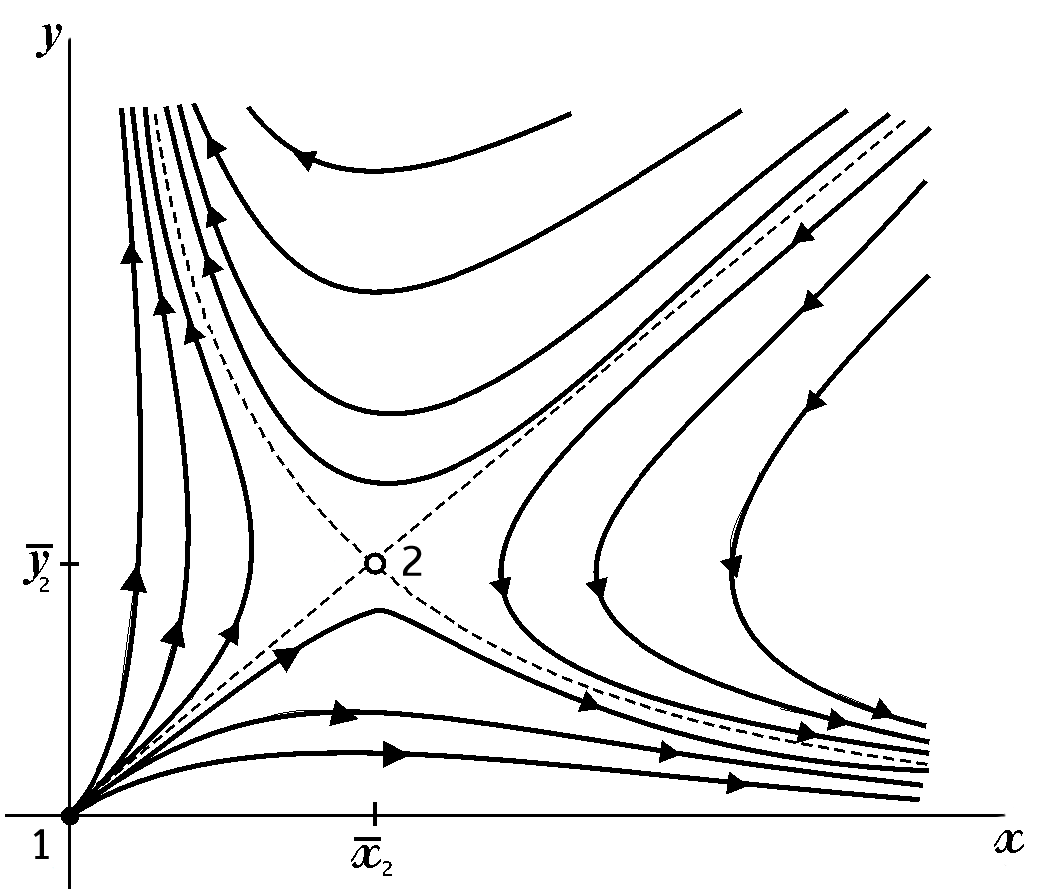
\includegraphics[width=.6\textwidth]{one_of_two_unlimited}
    \caption{Фазовый портрет системы}
    \label{phase_one_of_two}
\end{figure}

\vspace*{1em} % ----------------------------------------------------------------
\subsection{Отбор одного из нескольких равноправных}

Рассмотрим модель \eqref{common_model} в случае \( N \gg 1 \):
\begin{equation}
    \der{X_i}{t} = bX_i - \gamma\sum_{j = 1}^N X_i X_j + \gamma X_i^2 \quad
    \bigr(i = 1, 2, \ldots, N\bigl).
    \label{one_of_N}
\end{equation}

Введем безразмерные переменные \( t' = bt \) и \( x_i = \gamma X_i/b \). Тогда
система \eqref{one_of_N} перепишется в виде:
\begin{equation}
    \der{x_i}{t'} = x_i\left( 1 - \sum_{j = 1}^N x_j \right) + x_i^2 \qquad
    \bigl(i = 1, 2, \ldots, N\bigr).
    \label{one_of_N_ml}
\end{equation}

Свойства данной системы аналогичны \eqref{one_of_two_ml}: имеется \( N + 2 \)
стационарных состояний, в двух из которых все \( x_i \) принимают одинаковые
значения: в первом \( \st{x}_i = 0 \), во втором \( \st{x}_i = (N - 1)^{-1} \).
Остальные состояния соответствуют бесконечному значению одной из переменных и
нулевым значениям остальных.

\vspace*{2em} % ----------------------------------------------------------------
\section{Отбор одного из равноправных при ограниченном субстрате}

Неограниченный рост биомассы является недостатком простейшей модели, поэтому
учтем ограниченность питательных ресурсов. Рассмотрим субстрат \( S \),
лимитирующий рост популяции. Коэффициент репродукции \( a \) будет зависеть от
содержания субстрата \( S \): например, согласно выражению Моно
\begin{equation}
    a = \frac{a_0 S}{K_S + S}.
    \label{Mono}
\end{equation}

Интенсивность притока субстрата обозначим за \( v \). Расход субстрата
пропорционален поглощению его организмами, то есть сумме их концентраций.
Уравнение для скорости изменения концентрации субстрата во времени имеет вид:
\[
    \der{S}{t} = -\alpha a(X + Y) + v = -\alpha a_0 \frac{S}{K_S + S} + v,
\]
где экономическим коэффициентом \( \alpha > 1 \) учитывается, что не весь
поглощенный субстрат перерабатывается в биомассу, часть его пропадает.

Уравнения для концентраций объектов \( X \) и \( Y \) перепишем из
\eqref{one_of_two} с учетом ограниченности роста:
\begin{equation}
    \left\{ \begin{array}{l}
        \ds \der{X}{t} = a_0\frac{S}{K_S + S}X - \beta X - \gamma XY, \\[.3em]
        \ds \der{Y}{t} = a_0\frac{S}{K_S + S}Y - \beta Y - \gamma XY,
    \end{array} \right.
    \label{one_of_two_lim}
\end{equation}
где \( \beta \) -- коэффициент смертности, \( K_S \) -- концентрация субстрата,
при которой скорость роста равна половине максимальной. Объекты считаются
равноправными, следовательно, величины \( a_0 \), \( \beta \), \( K_S \) и
\( \gamma \) считаются одинаковыми для всех объектов.

Вводя безразмерные величины \( t' = \beta t \), \( x = \gamma X/\beta \),
\( y = \gamma Y/\beta \), \( s = \gamma S/\beta \), \( v' = v\gamma/\beta^2 \)
и обозначая \( k_s = \gamma K_S/\beta \), \( f(s) = a_0s/\beta(k_s + s) \),
перепишем систему в~виде:
\begin{equation}
    \left\{ \begin{array}{l}
        \ds \der{x}{t'} = f(s)x - x - xy, \\[.3em]
        \ds \der{y}{t'} = f(s)y - y - xy, \\[.3em]
        \ds \der{s}{t'} = -\alpha f(s)(x + y) + v'.
    \end{array} \right.
    \label{one_of_two_lim_ml}
\end{equation}

Принимая, что процессы поглощения и прибыли субстрата существенно быстрее, чем
процессы репродукции, то есть \( v' \gg 1 \) и \( \alpha \gg 1 \). Тогда третье
уравнение системы \eqref{one_of_two_lim_ml} преобразуется в алгебраическое
с \( \ds \der{s}{t'} = 0 \):
\[
    -\alpha f(s)(x + y) + v' = 0 \quad \text{или} \quad v' = \alpha f(s)(x + y);
\]
откуда имеем \( \ds f(s) = \frac{v'}{\alpha(x + y)} \). Подставляя найденный
вид функции в первые два уравнения системы \eqref{one_of_two_lim_ml} и
обозначая за \( v_0 = v'/\alpha \), получаем систему
\begin{equation}
    \left\{ \begin{array}{l}
        \ds \der{x}{t'} = x\left[\frac{v_0}{x + y} - (1 + y)\right], \\[.5em]
        \ds \der{y}{t'} = y\left[\frac{v_0}{x + y} - (1 + x)\right].
    \end{array} \right.
    \label{one_of_two_lim_ml_easy}
\end{equation}

Фазовый портрет такой системы приведен на рисунке \ref{phase_one_of_two_lim}.

\begin{figure}[h!]
    \centering
    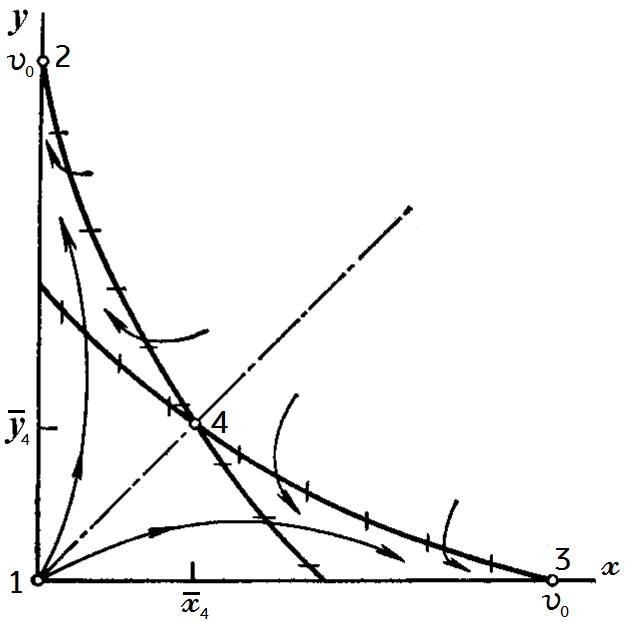
\includegraphics[width=.6\textwidth]{one_of_two_limited}
    \caption{Фазовый портрет системы}
    \label{phase_one_of_two_lim}
\end{figure}

Система \eqref{one_of_two_lim_ml_easy} имеет четыре стационарные точки:
\begin{enumerate}
    \item точка \( \st{x}_1 = \st{y}_1 = 0 \) -- неустойчивый узел,
    \item точка \( \st{x}_2 = 0 \) и \( \st{y}_2 = v_0 \) -- устойчивый узел,
    \item точка \( \st{x}_3 = v_0 \) и \( \st{y}_3 = 0 \) -- устойчивый узел,
    \item точка \( \st{x}_4 = \st{y}_4 = \cfrac{\sqrt{1 + 2v_0} - 1}{2} \) -- седло.
\end{enumerate}

Причиной отбора в этой системе, как и в системе \eqref{one_of_two}, является
неустойчивость симметричного стационарного состояния, появляющаяся в результате
антагонистического взаимодействия объектов. В такой системе выживет только один
из видов: \( X \) или \( Y \). Его стационарная концентрация
\( v_0 = v'/\alpha \) определяется скоростью притока субстрата и экономическим
коэффициентом.

При отсутствии взаимоподавления, то есть при \( \gamma \to 0 \), отбор
происходить не будет, обе популяции будут развиваться самостоятельно.

Увеличение же фактора взаимоподавления \( \gamma \) и интенсивности
источника \( v \) способствует отбору, а увеличение коэффициента смертности
\( \beta \) и неэффективности питания \( \alpha \) ведет к торможению отбора.

\vspace*{2em} % ----------------------------------------------------------------
\renewcommand{\bibname}{Список литературы}

\begin{thebibliography}{9} \addcontentsline{toc}{section}{Список литературы}
    \bibitem{1} Ризниченко, Г.Ю. Лекции по математическим моделям в 
            биологии. Ч.1. -- Ижевск: НИЦ
            <<Регулярная и хаотическая динамика>>, 2002, 232 с.
    \bibitem{2} Романовский, Ю.М. Математическое моделирование в биофизике
            -- Москва: <<Наука>>, 1975, 335 с.
\end{thebibliography}
\end{document}